\chapter{Introdução}
A maneira que temos de observar a natureza e o universo sempre dependeu de instrumentos, microscópios trouxeram a noção de que micro-organismos extremamente pequenos existiam, nos permitiram descobrir as bactérias, as formas de vida mais comuns do planeta, telescópios nos deram habilidades de observar o sistema solar descobrir as órbitas dos planetas e formular a noção de gravidade de Newton \cite{newton1687philosophiae}. 

Mas nem sempre essas descobertas aconteceram de propósito. Em 1930, o físico Karl Jansky foi encarregado de melhorar os sinais de rádio que cruzavam os oceanos com telégrafos e chamadas de telefone, para detectar de onde vinham as ondas de rádio que atrapalhavam a chamada com estática. Jansky construiu uma antena giratória que podia apontar para todas as direções. Foi quando ele descobriu ondas de rádio vindas de tempestades de raios próximas e distantes e uma terceira fonte de rádio no céu. O sinal ficava mais forte a cada 23 horas e 56 minutos, o tempo que as estrelas levam para percorrer o céu, o nosso dia sideral \cite{singh2010big}. 

O ponto que ele descobriu, era o centro da nossa Via Láctea, com a maior parte dos sinais de rádio vindos da constelação de sagitário. De alguma forma o universo estava cheio de fontes de ondas de rádio, uma descoberta por acaso, feita sem querer por alguém que estava preparado para entender o que havia encontrado, uma serendipidade. 
Assim como o sol emite radiação eletromagnética na forma de ondas de luz. Também emite frequências maior e menor, como rádio. Com apenas 26 anos, Jansky publicou o trabalho que inaugurou a radioastronomia, a observação do universo com os radiotelescópios, que nos permite ver, de explosões aos bips de pulsares \cite{jansky1932directional}. Como ver em outras ondas além da luz nos mostra novos fenômenos, observações de raio-x, por exemplo, mostram buracos negros rasgando as estrelas \cite{200814}, os quasares, em quanto a radiação infravermelha atravessa a Via Láctea e nos mostra o que tem por trás dela. 

E o que a descoberta da radioastronomia teve de serendipidade, a descoberta das ondas gravitacionais (Gravitational wave) (GW) teve de proposital. Começando por Einstein. Em 1915, quando ele adicionou a gravidade à teoria da relatividade, Publicando a "Teoria da Relatividade Geral" \cite{albert1920realtivity}, Einstein concluiu que a gravidade não era uma força, mas sim a deformação do espaço tempo, e essa deformação do espaço deveria viajar pelo universo como uma onda, viajando na velocidade da luz, mas isso só havia sido observado indiretamente. 

Por volta de 1960, descobertas astronômicas (quasares, pulsares, radiação cósmica de fundo) e novos experimentos impulsionaram a relatividade geral, para a linha de frente. Neste período foi descoberto a diminuição no período orbital do pulsar binário Hulse-Taylor em uma taxa consistente com a predição da relatividade geral da perda de energia por ondas gravitacionais \cite{weisberg2004relativistic}, e essa havia sido a primeira detecção indireta de ondas gravitacionais da historia da ciência, havia, por que agora, observamos pela primeira vez, dois buracos negros se fundindo e liberando uma energia 10 vezes maior do que a emissão de luz por todas as galáxias do universo observável. 

Pra isso precisamos do Observatório de Ondas Gravitacionais por Interferometria a Laser (Advanced Laser Interferometer Gravitational Wave Observatory) (aLIGO) \cite{PhysRevLett.116.131103,0264-9381-32-7-074001}, que recentemente, até o momento, tem anunciado a detecção de ondas gravitacionais a partir de medidas de uma série de eventos cósmicos que envolvem colapso de sistemas binários formados por objetos compactos tais como buracos negros \cite{abbott2016observation,ligo2016gw151226,scientific2017gw170104,abbott2017gw170814}, e estrelas de nêutrons \cite{abbott2017gw170817}, que são consistentes com as previsões gerais de relatividade de Einstein.

O observatório tem dois centros, com formato em L um posicionado em Washington e outro em Louisiana nos Estados Unidos, na quina desse L um espelho divide um feixe de laser em duas partes, que percorrem, cada uma, um dos tubos de 4 kilômetros e encontra um espelho lá no final, quando as ondas de laser voltam, se anulam e desaparecem se um dos tubos for deslocado por causa de uma deformação do espaço e do tempo, muda a distância percorrida pelo laser, e o sinal deixa de ser cancelado, como ilustra a Figura~\ref{figinterferometer}, pra garantir que a deformação foi causada por uma onda gravitacional e não um terremoto ou outro problema, o mesmo sinal tem que ser observado nos dois centros \cite{PhysRevLett.116.131103}. 

\begin{figure}[ht]
\centering
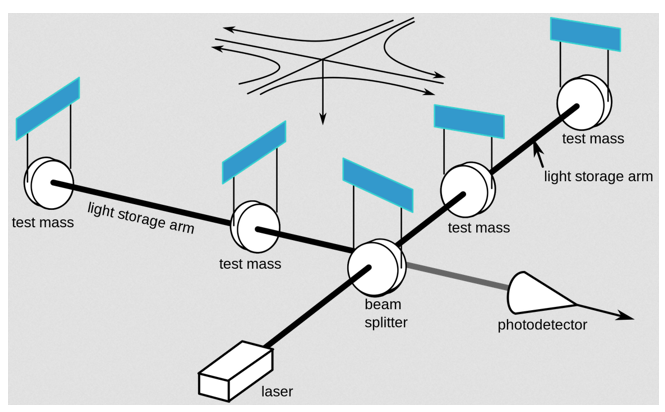
\includegraphics[width=1\textwidth]{figuras/interferometro.png}
\caption{Diagrama de um projeto básico de interferômetro. [Image: LIGO]}
\label{figinterferometer}
\end{figure}
 
Após a parada do LIGO nos periodos de 2010 à 2015 o observatorio foi parado para passar por um upgrade na capacidade de detecção e logo no inicio de suas atividade ele captou o primeiro sinal de uma colisão de buracos negros, há 1,3 bilhão de anos luz daqui, que levando ao prêmio Nobel de Física em 2017 \cite{abbott2016observation}. 
 
Quando um objeto denso e massivo é acelerado, ele cria ondas gravitacionais como as ondas que uma pedra lançada em um lago produz, e de acordo com Einstein, nada é mais denso e massivo do que um buraco negro. E o sistema binário, dois buracos negros giram um ao redor do outro, na primeira detecção que foi observada \cite{abbott2016observation}, um deles tinha a massa de 36 sóis e o outro de 29 conforme eles giram em órbita, emitem ondas gravitacionais e com isso perdem energia, conforme perdem energia, se aproximam ainda mais e giram ainda mais rápido quanto mais se aproximam, mais energia perdem e mais ondas emitem e mais se aproximam cada vez mais rápido até colidirem.

No final da explosão o buraco resultante ficou com 62 massas solares, os 3 sóis de diferença foram convertidos em ondas gravitacionais, conforme os buracos negros se aceleram antes da colisão, as ondas que emitem ficam cada vez mais intensas e cada vez mais frequentes, até virarem um gorjeio, que marca a colisão, um gorjeio emitido há mais de 1 bilhão de anos, uma explosão tão forte, que chacoalhou o espaço e o tempo e conseguimos captar daqui.

Agora temos a confirmação de que as ondas gravitacionais previstas há 100 anos existem, e sabemos como detectá-las. Em pouco tempo teremos detectores como LIGO em órbita da terra, com sensores há milhares de quilômetros de distância, capazes de detectar ondas gravitacionais ainda menores. Agora podemos captar as ondas emitidas pela explosão de supernovas ou pela fusão de estrelas de nêutrons formando buracos negros.


\section{Delimitação do Tema}

A natureza nem sempre pode ser observada em sua plenitude, mas sempre poderá ser simulada computacionalmente desde que existam os apropriados modelos computacionais. Neste sentido, a computação científica e numérica desempenha o papel de ferramenta fundamental da área da ciência da computação para o entendimento da natureza, explicitando fenômenos e dinâmicas muitas vezes não possíveis de serem observados pela limitada capacidade humana de observação.

Em particular, para a geração de modelos computacionais que venham a descrever a gravidade é necessário entender como o universo funciona. A teoria da Relatividade de Einstein \cite{albert1920realtivity} mostra que o espaço e o tempo não são entidades separadas. Desta forma, o espaço e o tempo formam um contínuum conhecido como espaço-tempo que participa da dinâmica dos eventos. As equações da Relatividade Geral de Einstein mostram que a dinâmica da matéria está conectada à curvatura do espaço-tempo. A gravidade é, portanto, uma manifestação da curvatura do espaço-tempo.

Um dos aspectos da dinâmica do espaço-tempo é radiação gravitacional. Prevista pela Teoria da Relatividade Geral em 1916, a descoberta das ondas gravitacionais tem sido um objetivo perseguido por cerca de 100 anos. A descoberta das ondas gravitacionais seria mais uma confirmação da Teoria da Relatividade Geral que se somaria às outras confirmações das Teoria de Einstein, tais como a deflexão da luz ao passar com objetos massivos como estrelas, lentes gravitacionais, a explicação do desvio do periélio do planeta Mercúrio, efeitos relativísticos nas órbirtas dos planetas, buracos negros, etc. 

Os efeitos Relativísticos de natureza gravitacionais são de grande importância à atual tecnologia e com aplicação à vida diária das pessoas. Um dos principais resultados da Teoria da Relatividade Geral foi a possibilidade de permitir a localização de coordenadas na superfície de planetas com extrema precisão (o equivalente ao georreferenciamento, contudo extraterrestre, a partir da Terra). A localização de coordenadas na superfície de planetas é uma das aplicações tecnológicas que só foi possível com uso da Teoria da Relatividade Geral. O resultado de tal tecnologia aplicado ao caso do planeta Terra foi o desenvolvimento da tecnologia do Sistema de Posicionamento Global GPS (Global Positioning System).

Por outro lado, a busca da detecção de ondas gravitacionais continua intensa, a análise e o tratamento computacional destas informações encontram-se na crisa da onda da tecnologia computacional para o entendimento de tal processo.

\section{Problema de Pesquisa}
Para que seja possível a detecção de GW é necessário um grande esforço contínuo dos detectores de GW e das instalações astronômicas e a natureza sensível a tempo dessas análises requer algoritmos que podem detectar e caracterizar eventos GW em tempo real e o custo computacional das buscas de filtros combinados aumenta significativamente quando se direciona as fontes de GW que abrangem um espaço de parâmetro dimensional mais alto.

A filtragem combinada, o algoritmo de detecção de GW mais sensível usado pelo LIGO, atualmente tem como alvo fontes binárias compactas com componentes alinhados à rotação em órbitas quase circulares.  Estudos recentes também indicam que essas buscas podem perder GWs geradas por populações binárias compactas formadas em ambientes estelares densos. Estender essas buscas com correspondência de modelos para direcionar BBHs de precessão por rotação, quase-circulares ou excêntricas é proibitivamente computacional \cite{george2018deep}.

Acelerar os algoritmos de estimação de parâmetros bayesianos offline, que normalmente duram de várias horas a alguns dias, não é uma tarefa trivial. a resposta para esses desafios tem sido o esforço continuo para reduzir o tamanho dos bancos de modelos usados para pesquisas GW baseadas em filtragem combinada \cite{indik2017reducing}. Com base nessas considerações, e percebendo que, para maximizar a ciência que se pode extrair das observações de GW, é essencial cobrir rapidamente um espaço de parâmetro mais profundo de fontes de motivação astrofísica, a comunidade da GW vem explorando instalações de computação de alto desempenho (HPC) de última geração para aumentar o conjunto de recursos computacionais para realizar a análise de dados GW em larga escala \cite{huerta2017boss,weitzel2017data}.


\section{Objetivos}
A seguir serão apresentados os objetivos geral (OG) e específicos (OE) que nortearão a condução desta pesquisa.

\subsection{Objetivo Geral}
A presente pesquisa tem como objetivo geral o desenvolvimento de procedimentos computacionais baseados em computação científica e numérica para o entendimento da dinâmica gravitacional do universo, contribuindo para uma nova área de pesquisa computacional designada de Astroinformatics com o desenvolvimento de bibliotecas computacionais para análise estatística dos resultados experimentais reais de medida das ondas gravitacionais. Para atingir esse objetivo geral foram propostos os objetivos específicos a seguir relacionados.
\subsection{Objetivos Específicos}
Para atingir o objetivo geral foram definidos os seguintes objetivos específicos: 
\begin{itemize}

\item Estudo introdutório dos processos de modelagem matemática para a geração das equações que governam as ondas gravitacionais;
\item Estudo das metodologias computacionais para a resolução de sistemas de equações diferenciais parciais acopladas;
\item E Desenvolvimento e implementação de bibliotecas numéricas para a solução de sistemas de equações diferenciais parciais em uma plataforma de GP/GPU (CUDA);
\item Simulações computacionais de ondas gravitacionais em uma plataforma baseada em GP/CPU (CUDA);
\item Estudo de inferência estatística e análise de ruídos para verificação de aderência entre os resultados obtidos pelo LIGO e as soluções numéricas obtidas.

\end{itemize}
\section{Justificativa}

Com base em todas as considerações descritas, precisamos de um novo paradigma para superar as limitações e os desafios computacionais dos algoritmos de detecção de GW existentes. Um candidato ideal seria a inteligencia artificial, mais especificamente as Machine Learning, a qual hoje é tendencia no mercado, que é uma área  altamente escalável que pode aprender diretamente a partir de dados brutos, sem qualquer recurso manual de engenharia, usando camadas hierárquicas profundas de “neurônios artificiais”. redes, em combinação com técnicas de otimização baseadas em retro-propagação e gradiente descendente \cite{barca2005treinamento}. A Machine Learning, especialmente com o auxílio da computação GPU, alcançou recentemente um imenso sucesso em aplicações comerciais e em inteligência artificial \cite{esteva2017dermatologist}, \cite{moravvcik2017deepstack}, \cite{van2016wavenet}, \cite{10.1007/978-3-319-44188-7_16}, e também tem sido aplicado em astrofísica \cite{george2017glitch}, \cite{george2017deepA}.